\documentclass[
  a4paper,
  11pt,
]{scrartcl}

\usepackage[utf8]{inputenc}
\usepackage[
  %cm,
  headings
]{fullpage}
\usepackage[ngerman]{babel}
\usepackage{amsmath}
\usepackage{amssymb}
\usepackage{amsthm}

\theoremstyle{plain}
\newtheorem{satz}{Satz}
\theoremstyle{definition}
\newtheorem{definition}{Definition}
\theoremstyle{remark}
\newtheorem{beispiel}{Beispiel}

%\usepackage{minted}
\usepackage{listings}
\usepackage{tikz}
\usepackage{pgfplots}
\usepackage{booktabs}
\usepackage{hyperref}
\usepackage{abstract}

\usepackage[]{algorithm}
\usepackage[]{algorithmic}
\floatname{algorithm}{Algorithmus}

% Für Zeilenumbrüche ohne Indentations
% \setlength{\parindent}{0pt}

% coole Kopf- und Fußzeilen:
\usepackage{fancyhdr}
% Seitenstil ist natürlich fancy:
\pagestyle{fancy}
% alle Felder löschen:
\fancyhf{}

\fancyhead[L]{%
  Seminar: Public-Key-Kryptographie
}
\fancyhead[R]{%
}
%\fancyfoot[L]{}
\fancyfoot[C]{\thepage}

\usepackage{todonotes}

\newcommand{\N}{\mathbb{N}}
\newcommand{\Z}{\mathbb{Z}}
\renewcommand{\P}{\mathbb{P}}
\newcommand{\ggT}{\text{ggT}}
\newcommand{\Mod}[1]{\ \mathrm{mod}\ #1}

\usepackage{tabularx} % tabellen hannes
\def\doubleunderline#1{\underline{\underline{#1}}} % doppelt unterstrichen: \doubleunderline{abc}

\title{Diskrete Logarithmen}

\subtitle{Seminar: Public-Key-Kryptographie}

\author{%
  Martin Darmüntzel \and Hannes Kleinwort
}

\begin{document}

\maketitle

\begin{abstract}
  Diese Ausarbeitung gibt einen Überblick über das diskrete Logarithmusproblem
  und geht dabei auf die wichtigsten mathematischen Grundlagen, die Anwendung
  beim Schlüsselaustausch bzw. der Verschlüsselung und mögliche
  Berechnungsmethoden ein.
\end{abstract}

\tableofcontents

\section{Mathematische Grundlagen}
\label{sec:mathematische_grundlagen}
  Wir setzen voraus, dass die Leser mit den wichtigsten Begriffen und Sätzen der
  Gruppen- bzw. Zahlentheorie vertraut sind.
  Dazu zählen wir die Definition der
  Gruppe und der Kongruenzrechnung,
  den (erweiterten) Euklidischen Algorithmus,
  das Lemma von Bézout,
  die Eulersche $\varphi$-Funktion,
  den kleinen Satz von Fermat,
  den Satz von Lagrange
  und
  den Chinesischen Restsatz.

\begin{definition}[Prime Restklassengruppe]
  Die \emph{prime Restklassengruppe} ist die multiplikative Gruppe der
  Restklassen bezüglich eines Moduls $p$, die zu $p$ teilerfremd sind. Sie wird
  als $\Z_p^*$ notiert.
\end{definition}

Die Bedingung der Teilerfremdheit der einzelnen Elemente $a \in \Z_p^*$ zum
Modul $p$ drückt sich durch $\ggT(a, p) = 1$ für alle $a \in \Z_p^*$ aus. Durch
diese Bedingung und dem Lemma von Bézout hat jedes Element ein multiplikatives
Inverses in $\Z_p^*$. Falls $p$ eine Primzahl ist, dann besteht $\Z_p^*$ aus
der Menge $\left\{1, \ldots, p-1\right\}$, da alle Zahlen aus dieser Menge
teilerfremd zu $p$ sind. Im Allgemeinen ist die Ordnung von $\Z_p^*$ durch die
Eulersche $\varphi$-Funktion bestimmt:
\begin{align*}
  \left| \Z_p^* \right| = \varphi(p)
\end{align*}
Dies ergibt sich direkt aus der Definition der Eulerschen $\varphi$-Funktion.

\begin{definition}[Erzeuger]\label{def:erzeuger}
  Wenn es ein Element $a \in \Z_p^*$ gibt, dessen Potenzen $a^n$ für
  $n \in \Z_p^*$ alle Elemente aus $\Z_p^*$ erzeugt, dann nennt man $a$ einen
  Erzeuger. In $\Z_p^*$ heißen die Erzeuger auch \emph{Primitivwurzeln} modulo
  $p$.
\end{definition}

\begin{beispiel}[Erzeuger]\label{bsp:erzeuger}
  Betrachten wir $\Z_{13}^*$. In dieser Gruppe ist $2$ ein Erzeuger, was man
  durch das Ausrechnen der einzelnen Potenzen überprüfen kann:
  \begin{center}
    \begin{tabular}{r*{12}{r}}
      \toprule
      $x$ & $1$ & $2$ & $3$ & $4$ & $5$ & $6$ & $7$ & $8$ & $9$ & $10$ & $11$ & $12$\\
      \midrule
      $2^x \Mod{13}$ & $2$ & $4$ & $8$ & $3$ & $6$ & $12$ & $11$ & $9$ & $5$ & $10$ & $7$ & $1$\\
      \bottomrule
    \end{tabular}
  \end{center}
  Das Element $3$ ist hingegen kein Erzeuger:
  \begin{center}
    \begin{tabular}{r*{12}{r}}
      \toprule
      $x$ & $1$ & $2$ & $3$ & $4$ & $5$ & $6$ & $7$ & $8$ & $9$ & $10$ & $11$ & $12$\\
      \midrule
      $3^x \Mod{13}$ & $3$ & $9$ & $1$ & $3$ & $9$ & $1$ & $3$ & $9$ & $1$ & $3$ & $9$ & $1$\\
      \bottomrule
    \end{tabular}
  \end{center}
\end{beispiel}

Um herauszufinden, ob ein Element $a \in \Z_p^*$ eine Primitivwurzel ist, müsste
man testen, ob die Potenzen $a^x$ mit $x \in \Z_p^*$ wieder alle Elemente von
$\Z_p^*$ ergeben. Dies ist für große Moduli jedoch sehr aufwändig. Wir können
diesen Test abkürzen, indem wir uns folgende Beobachtung aus
Beispiel~\ref{bsp:erzeuger} zunutze machen: nach dem kleinen Satz von Fermat
muss für jedes Element $a$ aus $\Z_p^*$ die Kongruenz
\begin{align*}
  a^{p-1} \equiv 1 \Mod{p}
\end{align*}
gelten. Für das Element $3 \in \Z_{13}^*$ gilt sie jedoch auch für die
Exponenten $3, 6$ und $9$. Wir müssen demnach nur für bestimmte Exponenten $x$
prüfen, ob $a^x \equiv 1 \Mod{p}$ gilt und falls das der Fall ist, kann $a$ keine
Primitivwurzel sein. Welche Exponenten dies sind, zeigt der folgende Satz.

\begin{satz}\label{satz:primitivwurzeltest}
  Sei $p$ eine Primzahl größer als $2$ und
  $p-1 = q_1^{k_1} \cdot \ldots \cdot q_r^{k_r}$ die Primfaktorzerlegung von
  $p-1$. Eine ganze Zahl $a$ mit $p \nmid a$ ist genau dann Primitivwurzel
  modulo $p$, wenn
  \begin{align*}
    a^{(p-1)/q_i} & \not\equiv 1 \Mod{p} \qquad \text{ für alle } i \in \left\{1, \ldots, r\right\}.
  \end{align*}

  \begin{proof}
    \begin{itemize}
      \item[„$\Rightarrow$“] Durch die Definition der Primitivwurzel modulo $p$
        und dem kleinen Satz von Fermat darf eine Potenz $a^n$ mit
        $n \in \Z_p^*$ nur für den Fall $n = p-1$ kongruent zu $1$ sein. Wäre
        sie es für ein anderes $n$, dann wäre $a$ keine Primitivwurzel.
      \item[„$\Leftarrow$“] Sei $m$ die Ordnung von $a \Mod{p}$ in $\Z_p^*$.
        Nach dem Satz von Lagrange gilt $m \mid (p-1)$. Wenn $m < p-1$ wäre,
        dann müsste es einen Primteiler $q_i \mid (p-1)$ geben, so dass
        $m \mid (p-1)/q_i$, woraus folgt $a^{(p-1)/q_i} \equiv 1 \Mod{p}$. Dies
        ist ein Widerspruch zur Voraussetzung. Demnach hat $a$ die Ordnung
        $m = (p-1)$ und ist Primitivwurzel.
    \end{itemize}
  \end{proof}
\end{satz}

\begin{beispiel}[Primitivwurzel testen]\label{bsp:primitivwurzel_testen}
  Betrachten wir $p = 73 = 2^3 \cdot 3^2 + 1$ und untersuchen mit
  Satz~\ref{satz:primitivwurzeltest}, ob $r_1 = 2, r_2 = 3$ und $r_3 = 5$
  Primitivwurzeln sind.

  \begin{description}
    \item[$r_1 = 2$:]
      \begin{align*}
        2^{72/2}
        & \equiv 2^{36} \equiv 1 \Mod{p}
      \end{align*}
      Damit ist $2$ keine Primitivwurzel.
    \item[$r_2 = 3$:]
      \begin{align*}
        3^{72/2}
        & \equiv 3^{36} \equiv 1 \Mod{p}
      \end{align*}
      Damit ist auch $3$ keine Primitivwurzel.
    \item[$r_3 = 5$:]
      \begin{align*}
        5^{72/2}
        & \equiv 5^{36} \equiv 72 \Mod{p}\\
        5^{72/3}
        & \equiv 5^{24} \equiv 8 \Mod{p}\\
      \end{align*}
      Damit ist $5$ eine Primitivwurzel modulo $73$.
  \end{description}
\end{beispiel}

Mit Satz~\ref{satz:primitivwurzeltest} können wir effizienter eine
Primitivwurzel finden. Wenn wir eine solche gefunden haben, können wir sogar
alle anderen Primitivwurzeln mit dem folgenden Satz bestimmen.

\begin{satz}\label{satz:primitivwurzeln_durch_potenzen}
  Sei $a$ eine Primitivwurzel von $\Z_p^*$. Es ist $a^k$ genau dann eine
  Primitivwurzel von $\Z_p^*$, wenn $k$ und $p-1$ (die Ordnung von $\Z_p^*$)
  teilerfremd sind.

  \begin{proof}
    \begin{itemize}
      \item[„$\Rightarrow$“] Wir setzen $b := a^k$ und nehmen an, dass $k$ und
        $p-1$ teilerfremd sind. Dann gibt es nach dem Lemma von Bézout ganze
        Zahlen $s, t$ mit $s k + t (p-1) = 1$. Daraus folgt
        \begin{align*}
          b^s \equiv a^{k s} \equiv a^{1 - t (p-1)} \equiv a \Mod{p},
        \end{align*}
        da
        \begin{align*}
          a^{- t (p-1)} \equiv {\left(a^{(p-1)}\right)}^{-t} \equiv 1^{-t} \equiv 1 \Mod{p}
        \end{align*}
        Mittels $b$ kann demnach die Primitivwurzel $a$ erzeugt werden, sodass
        $b$ selbst alle Elemente von $\Z_p^*$ erzeugen kann. Damit ist $b$ eine
        Primitivwurzel.
      \item[„$\Leftarrow$“] Sei wieder $b := a^k$. Wir nehmen an, dass $b$ eine
        Primitivwurzel von $\Z_p^*$ ist. Dann gibt es ein Element
        $s \in \Z_p^*$, so dass $b^s \equiv a \Mod{p}$. Also ist
        $a^{ks} \equiv a \Mod{p}$, woraus $a^{ks - 1} \equiv 1 \Mod{p}$ folgt.
        Demnach muss $ks-1$ ein Vielfaches der Gruppenordnung $p-1$ sein, sodass
        es eine ganze Zahl $t$ mit
        \begin{align*}
          ks - 1 = t(p-1)
        \end{align*}
        geben muss. Dies bedeutet aber, dass $k$ und $p-1$ teilerfremd sein
        müssen.
    \end{itemize}
  \end{proof}
\end{satz}

Da $\Z_p^*$ die Ordnung $\varphi(p) = p-1$ hat und die Anzahl der teilerfremden
Zahlen zu $p-1$ gleich $\varphi(p-1)$ ist, hat $\Z_p^*$ insgesamt
$\varphi(\varphi(p))$ Primitivwurzeln.

\begin{beispiel}[weitere Primitivwurzeln finden]
  Wir betrachten $\Z_{17}^*$ mit dem Erzeuger $3$. Mit
  Satz~\ref{satz:primitivwurzeln_durch_potenzen} wollen wir weitere
  Primitivwurzeln bestimmen.

  Die Menge der zu $p-1 = 16$ teilerfremden Zahlen ist
  \begin{align*}
    \left\{1, 3, 5, 7, 9, 11, 13, 15 \right\}.
  \end{align*}
  Damit erhalten wir die Primitivwurzeln:
  \begin{align*}
    3^1 & \equiv 3 \Mod{17}\\
    3^3 & \equiv 10 \Mod{17}\\
    3^5 & \equiv 5 \Mod{17}\\
    3^7 & \equiv 11 \Mod{17}\\
    3^9 & \equiv 14 \Mod{17}\\
    3^{11} & \equiv 7 \Mod{17}\\
    3^{13} & \equiv 12 \Mod{17}\\
    3^{15} & \equiv 6 \Mod{17}\\
  \end{align*}
  Die Menge der Primitivwurzeln von $\Z_{17}^*$ ist somit
  $\left\{ 3, 5, 6, 7, 10, 11, 12, 14 \right\}$.
\end{beispiel}

\begin{definition}[Diskrete Exponentiation, diskreter Logarithmus]
  Sei $g$ ein Erzeuger von $\Z_p^*$. Die diskrete Exponentiation zur Basis $g$
  ist eine Abbildung von $\Z_p^* \to \Z_p^*$ und definiert durch:
  \begin{align*}
    \exp_g: \quad \Z_p^* \to \Z_p^*\\
    x \mapsto g^x
  \end{align*}
  Die dazugehörige Umkehrfunktion
  \begin{align*}
    \log_g: \quad \Z_p^* & \to \Z_p^*\\
    x & \mapsto \log_g x
  \end{align*}
  heißt \emph{diskreter Logarithmus} zur Basis $g$.
\end{definition}

\begin{definition}[Diskretes Logarithmusproblem]\label{def:diskretes_logarithmusproblem}
  Sei $p$ eine Primzahl, $g$ ein Erzeuger von $\Z_p^*$ und $y \in \Z_p^*$.
  Finde ein $x$ mit $1 \leq x \leq p-1$, so dass $g^x \equiv y \Mod{p}$ gilt.
\end{definition}

Zum Schluss noch zwei Sätze zur Kongruenzrechnung, die später beim
Dif"-fie-Hell"-man-Schlüs"-sel"-aus"-tausch (Abschnitt~\ref{sub:dhke_proof})
benötigt werden.

\begin{satz}\label{satz:multiplikation_modulo}
  Seien $a,b,c,d \in \Z$ und $m \in \N$ mit $a \equiv b \mod m$ und $c \equiv d
  \mod m$. Dann gilt
  \begin{align*}
    a \cdot c \equiv b \cdot d \mod m
  \end{align*}
  \begin{proof}
    Aus $a \equiv b \Mod{m}$ und $c \equiv d \Mod{m}$ folgt aus der Definition
    der Kongruenz, dass $x, y \in \Z$ mit $b = a+mx$ und $d = c+my$ existieren.
    Dann ist $bd = ac + (ay + cx + mxy) \cdot m$, woraus $ac \equiv bd \Mod{m}$
    folgt.
  \end{proof}
\end{satz}

\begin{satz}\label{satz:potenzen_bei_kongruenzen}
  Seien $a, b \in \Z$ und $m \in \N$ mit $a \equiv b \Mod{m}$, dann gilt für
  alle $k \in \N$ mit $k \geq 1$:
  \begin{align*}
    a^k \equiv b^k \mod m
  \end{align*}
  \begin{proof}
    Ergibt sich aus der wiederholten Anwendung von
    Satz~\ref{satz:multiplikation_modulo} mit $c = a$ und $d = b$.
  \end{proof}
\end{satz}

\section{Anwendung: Ver- und Entschlüsselung}
\label{sec:anwendung_ver_und_entschlusselung}

\subsection{Diffie-Hellman-Merkle Schlüsselaustausch (DHKE)}
\label{sub:diffie_hellman_key_exchange}

Der auf der Schwierigkeit des Diskreten-Logarithmus-Problems beruhende
Diffie-Hellman-Merkle-Schlüsselaustausch, englisch:
\textbf{D}iffie-\textbf{H}ellman-\textbf{K}ey-\textbf{E}xchange (\textbf{DHKE}),
hat den folgenden Ablauf:
Zwei Kommunikationspartner, hier Alice und Bob, kommunizieren über einen
unsicheren Kanal und wollen einen Schlüssel für eine sichere Kommunikation,
z.\,B. durch eine symmetrische Verschlüsselung, austauschen.

Im ersten Schritt wählt Alice eine ausreichend große Primzahl $p$, welche den
bekannten Fallstricken des Verfahrens ausweicht, z.\,B. mit $p = c \cdot q+1$,
$c \in \N \setminus \{ 0 \}$, $q$ prim, $q$ möglichst groß (etwa
$p = 2 \cdot q + 1$).
Ausreichend groß bedeutet hierbei, dass die Bitlänge $n$ der Primzahl $p$
so groß ist, dass die Berechnung des diskreten Logarithmus $\text{DL}(y,g,p)$
mit bekannten Algorithmen und aktueller Hardware auf absehbare Zeit nicht
möglich sein wird (siehe Abschnitt~\ref{ssub:komplexitaet_naiver_algorithmus}).
Zur Zeit kann für $p$ eine Bitlänge von $n_p = 2048$ und für $q$ eine Bitlänge
von $n_q = 256$ als sicher angenommen werden.
Weiterhin bestimmt Alice eine Primitivwurzel $g \in \Z_p^*$ (siehe
Abschnitt~\ref{def:erzeuger}).
Dann wählt Alice ihren geheimen privaten Schlüssel
$a \in \Z_p^*$, $(1 \leq a \leq p-2)$, berechnet ihren öffentlichen Schlüssel
$A$ mit $A \equiv g^a \mod p$ und sendet $(g, p, A)$ über den unsicheren Kanal
an Bob.

Im zweiten Schritt wählt Bob seinen geheimen privaten Schlüssel $b \in \Z_p^*$,
$(1 \leq b \leq p-2)$, berechnet seinen öffentlichen Schlüssel $B$ mit
$B \equiv g^b \mod p$ und sendet $B$ über den unsicheren Kanal an Alice.
Der gemeinsame geheime Schlüssel $K$ ergibt sich nun auf der Seite von Alice mit
\begin{align*}
  K \equiv B^a \Mod{p}
\end{align*}
und auf der Seite von Bob mit
\begin{align*}
  K \equiv A^b \Mod{p} \text{.}
\end{align*}

\begin{figure}[H]
  \centering
  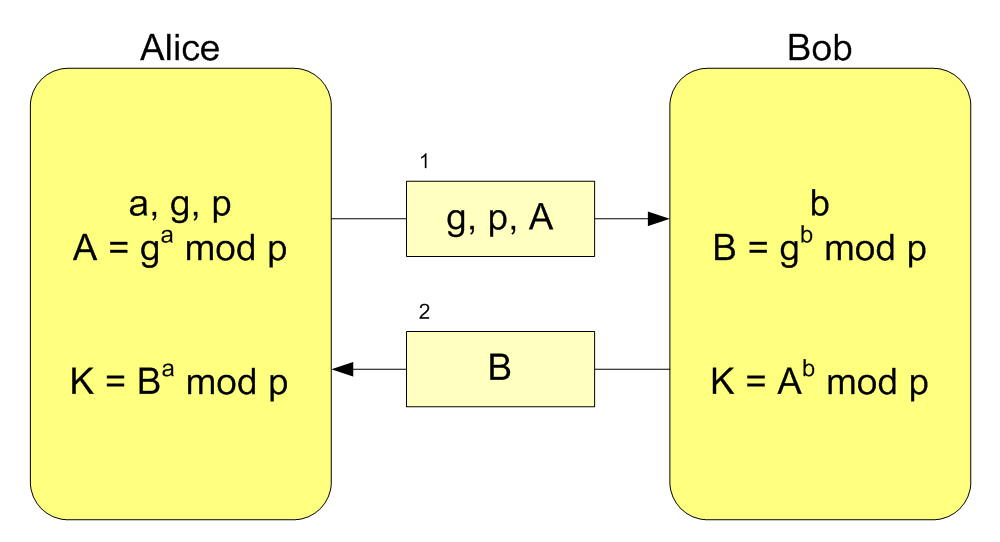
\includegraphics[width=\textwidth]{Diffie-Hellman-Schluesselaustausch2.png}
  \caption{Diffie-Hellman-Merkle-Schlüsselaustausch}
  \label{fig:dhke}
\end{figure}

\subsubsection{Korrektheit: Diffie-Hellman-Merkle Schlüsselaustausch (DHKE)}
\label{sub:dhke_proof}
Zur Korrektheit des Diffie-Hellman-Merkle Schlüsselaustausches: Beide
Kommunikationspartner haben den gleichen Schlüssel $K = K_1 = K_2$:

Mit der Kongruenz aus Satz~\ref{satz:potenzen_bei_kongruenzen} lässt sich
zeigen, dass die Schlüssel $K_1$ von Alice und $K_2$ von Bob kongruent sind:
\begin{align*}
  K_1 & \equiv B^a \Mod{p}\\
  & \equiv {(g^b)}^a \Mod{p}\\
  & \equiv g^{b \cdot a} \Mod{p}\\
  & \equiv g^{a \cdot b} \Mod{p}\\
  & \equiv {(g^a)}^b \Mod{p}\\
  & \equiv A^b \Mod{p}\\
  & \equiv K_2
\end{align*}

\subsubsection{Beispiel: Diffie-Hellman-Merkle Schlüsselaustausch (DHKE)}
\label{sub:dhke_beispiel}
\begin{beispiel}[Diffie-Hellman-Merkle Schlüsselaustausch]\label{bsp:dhke}
  Die zwei Kommunikationspartner Alice und Bob tauschen einen gemeinsamen
  geheimen Schlüssel $K$ über einen unsicheren Kanal aus (zu Anschauungszwecken
  mit kleinen Primzahlen). Alice kann Schritt 1 lange vor dem Schlüsselaustausch
  durchführen und das Ergebnis auf einem Schlüsselserver, wie z.B.
  \url{https://sks-keyservers.net}, veröffentlichen.
  \begin{center}
    \begin{tabularx}{\textwidth}{lXr}
      \textbf{Alice} & & \textbf{Bob}\\
      \midrule
    \end{tabularx}
    \begin{tabularx}{\textwidth}{lXcXl}
      \textbf{Schritt 1:} & & & & \\
      & & & & \\
      $\cdot$ wähle Primzahl: $\underline{p = 17}$ & & & & \\
      & & & & \\
      $\cdot$ finde Erzeuger: $\underline{g = 5}$ & & & & \\
      & & & & \\
      $\cdot$ wähle geheimen Schlüssel: & & & & \\
      $a \in \{1, \dots, p-2\}$ & & & & \\
      $\underline{a = 10}$ & & & & \\
      & & & & \\
      $\cdot$ berechne öffentlichen Schlüssel: & & & & \\
      $A \equiv g^a \Mod{p}$ & & & & \\
      $A = 5^{10} \Mod{17}$ & & & & \\
      $\underline{A = 9}$ & & & & \\
      & & & & \\
      $\cdot$ sende an Bob bzw. veröffentliche: & & & & \\
      $(g = 5, p = 17, A = 9)$ & & $\to$ & & \\\midrule
    \end{tabularx}
    \begin{tabularx}{\textwidth}{lXcXl}
      & & & & \textbf{Schritt 2}:\\
      & & & & \\
      & & & & $\cdot$ wähle geheimen Schlüssel:\\
      & & & & $b \in \{1, \dots, p-2\}$\\
      & & & & $\underline{b=7}$\\
      & & & & \\
      & & & & $\cdot$ berechne öffentlichen Schlüssel:\\
      & & & & $B \equiv g^b \Mod{p}$\\
      & & & & $B = 5^7 \Mod{17}$\\
      & & & & $\underline{B = 10}$\\
      & & & & \\
      & & & & $\cdot$ sende an Alice:\\
      & & $\leftarrow$ & & $(B=10)$ \\\midrule
    \end{tabularx}
    \begin{tabularx}{\textwidth}{lXcXl}
      & & \textbf{Schritt 3}: & & \\
      & & $\cdot$ berechne geheimen Schlüssel $K$: & & \\
      $K_1 \equiv B^a \Mod{p}$ & & & & $K_2 \equiv A^b \Mod{p}$\\
      $K_1 = 10^{10} \Mod{17}$ & & & & $K_2 = 9^7 \Mod{17}$\\
      $\doubleunderline{K_1 = 2}$ & & & & $\doubleunderline{K_2 = 2}$\\
      & & $\doubleunderline{K_1 = K = K_2}$ & &\\\midrule
    \end{tabularx}
  \end{center}
  Der geheime Schlüssel $K$, den nur Alice und Bob kennen, ist für einen
  Mithörer der öffentlichen Kommunikation nur schwierig zu ermitteln, da dieser
  den diskreten Logarithmus $\text{DL}(A,g,p) = a$ als Lösung der Gleichung
  $A \equiv g^a \Mod{p}$ bzw. $\text{DL}(B,g,p) = b$ als Lösung der Gleichung
  $B \equiv g^b \Mod{p}$ berechnen muss, um $K_1 \equiv B^a \Mod{p}$ oder
  $K_2 \equiv A^b \Mod{p}$ ermitteln zu können (siehe Abschnitt~\ref{ssub:komplexitaet_naiver_algorithmus}).
\end{beispiel}

\subsection{Verschlüsselung mittels Diffie-Hellman-Merkle-Schlüsselaustausch}
\label{sub:enc_with_dhke}
Ein Kommunikationspartner (Bob) schickt eine geheime Nachricht $m$ an einen
anderen Kommunikationspartner (Alice) über einen unsicheren Kanal durch
Verschlüsselung mittels
\textbf{D}iffie-\textbf{H}ellman-\textbf{K}ey-\textbf{E}xchange (DHKE). Bevor,
möglicherweise lange bevor, Bob eine Nachricht an Alice schicken möchte, muss
diese Ihren öffentlichen Schlüssel in geeigneter Weise auf einem Schlüsselserver
veröffentlichen, wie z.B. \url{https://sks-keyservers.net}. Des Weiteren
gleichen sich die Verfahren des DHKE und die Verschlüsselung mittels DHKE, wobei
Bob den öffentlichen Schlüssel von Alice beim Schlüsselserver erfragt. An der
Stelle der Erzeugung des geheimen Schlüssels $K$ bei DHKE verschlüsselt Bob dann
stattdessen die Nachricht $m$ zum Chiffretext $c$, mit $c \equiv A^b \cdot m
\Mod{p}$, und sendet $c$ zusammen mit seinem öffentlichen Schlüssel $B$ an ein
Postfach von Alice. Alice entschlüsselt die Nachricht dann mit $m \equiv
B^{-a}\cdot c  \Mod{p}$, was nach dem kleinen Satz von Fermat (siehe
Abschnitt~\ref{def:erzeuger}) kongruent ist zu $m \equiv B^{(p-1)-a}\cdot c
\Mod{p}$.

\begin{figure}[H]
  \centering
  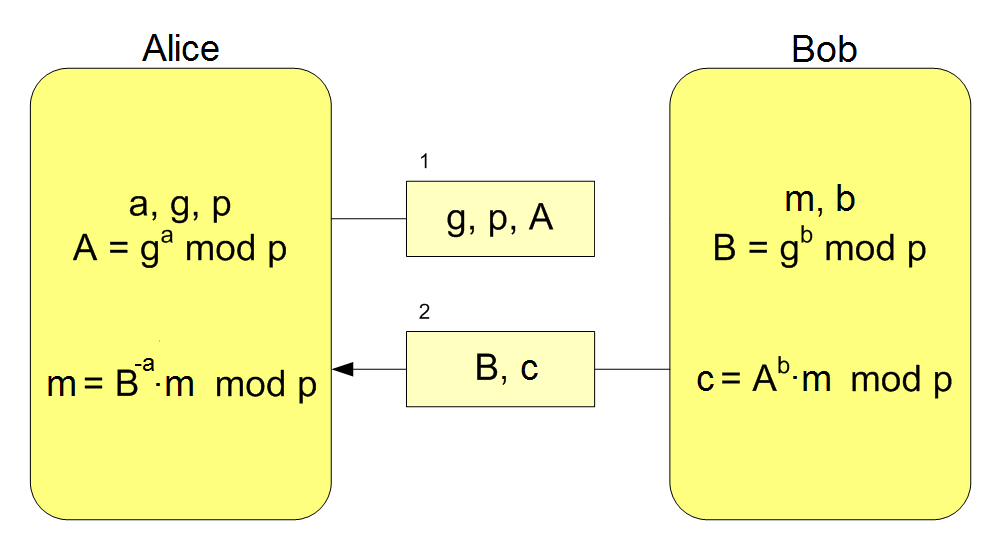
\includegraphics[width=\textwidth]{DHKE_enc.png}
  \caption{Verschlüsselung mittels Diffie-Hellman-Merkle-Schlüsselaustausch}
  \label{fig:enc_with_dhke}
\end{figure}

\subsubsection{Korrektheit: Verschlüsselung mittels DHKE}
\label{sub:enc_with_dhke_proof}
Beide Kommunikationspartner haben die gleiche Nachricht: $m = m_{\text{Bob}} =
m_{\text{Alice}}$
\begin{proof}
	Mit der Satz~\ref{satz:potenzen_bei_kongruenzen} lässt sich zeigen, dass
	\begin{align*}
      m_{\text{Alice}} & \equiv B^{-a} \cdot c \Mod{p}\\
      & \equiv (g^b)^{-a} \cdot c \Mod{p}\\
      & \equiv g^{b \cdot (-a)} \cdot c \Mod{p}\\
      & \equiv g^{-ab} \cdot c \Mod{p}\\
      & \equiv g^{-ab} \cdot A^b \cdot m_{\text{Bob}} \Mod{p}\\
      & \equiv g^{-ab} \cdot (g^a)^b \cdot m_{\text{Bob}} \Mod{p}\\
      & \equiv g^{-ab} \cdot g^{ab} \cdot m_{\text{Bob}} \Mod{p}\\
      & \equiv g^{-ab+ab} \cdot m_{\text{Bob}} \Mod{p}\\
      & \equiv m_{\text{Bob}}
    \end{align*}
\end{proof}

\subsubsection{Beispiel: Verschlüsselung mittels DHKE}
\label{sub:enc_with_dhke_example}
\begin{beispiel}[Verschlüsselung mittels Diffie-Hellman-Merkle Schlüsselaustausch]
  Bob schickt eine geheime Nachricht $M$ über einen unsicheren Kanal an Alice.
  Dazu muss er zuerst die Textnachricht als Zahlennachricht $m$ kodieren.
  Alice kann Schritt 1 womöglich lange vor dem Senden der Nachricht durchführen
  und ihren öffentlichen Schlüssel auf einem Schlüsselserver, wie z.B.
  \url{https://sks-keyservers.net}, veröffentlichen.
  \begin{center}
    \begin{tabularx}{\textwidth}{lXr}
      \textbf{Alice} & & \textbf{Bob}\\
      \midrule
    \end{tabularx}
    \begin{tabularx}{\textwidth}{lXcXl}
      \textbf{Schritt 1:} & & & & \\
      & & & & \\
      $\cdot$ wähle Primzahl: $\underline{p = 47}$ & & & & \\
      & & & & \\
      $\cdot$ finde Erzeuger: $\underline{g = 5}$ & & & & \\
      & & & & \\
      $\cdot$ wähle geheimen Schlüssel: & & & & \\
      $a \in \{1, \dots, p-2\}$ & & & & \\
      $\underline{a = 9}$ & & & & \\
      & & & & \\
      $\cdot$ berechne öffentlichen Schlüssel: & & & & \\
      $A \equiv g^a \Mod{p}$ & & & & \\
      $A = 5^{9} \Mod{47}$ & & & & \\
      $\underline{A = 40}$ & & & & \\
      & & & & \\
      $\cdot$ sende an Bob bzw. veröffentliche: & & & & \\
      $(g = 5, p = 47, A = 40)$ & & $\to$ & &\\\midrule
    \end{tabularx}
    \begin{tabularx}{\textwidth}{lXcXl}
      & & & & \textbf{Schritt 2}:\\
      & & & & \\
      & & & & $\cdot$ wähle geheimen Schlüssel:\\
      & & & & $b \in \{1, \dots, p-2\}$\\
      & & & & $\underline{b=13}$\\
      & & & & \\
      & & & & $\cdot$ berechne öffentlichen Schlüssel:\\
      & & & & $B \equiv g^b \Mod{p}$\\
      & & & & $B = 5^{13} \Mod{47}$\\
      & & & & $\underline{B = 43}$\\
      & & & & \\
      & & & & $\cdot$ kodiere Klartext als Zahlen:\\
      & & & & $\text{A} \mapsto 1, \text{B} \mapsto 2, \ldots, \text{Z} \mapsto 26, \textvisiblespace \mapsto 27$\\
      & & & & $M =(\text{KOMME MORGEN}) \mapsto $\\
      & & & & $\underline{(11, 15, 13, 13, 5, 27, 13, 15, 18, 7, 5, 14) = m}$\\
      & & & & \\
      & & & & $\cdot$ verschlüssele Klartext:\\
      & & & & $c_j \equiv A^b \cdot m_j \Mod{p}$\\
      & & & & $c_1 \equiv 22 \cdot 11 \Mod{47}$\\
      & & & & $c_1 \equiv 7$\\
      & & & & $c_2 \equiv 22 \cdot 15 \Mod{47}$\\
      & & & & $c_2 \equiv 1$\\
      & & & & $\dots$\\
      & & & & $\text{enc(m)} \mapsto$\\
      & & & & $\underline{(7, 1, 4, 4, 16, 30, 4, 1, 20, 13, 16, 26) = c}$\\
      & & & & \\
      & & & & $\cdot$ sende an Alice:\\
      & & $\leftarrow$ & & $(B, c)$\\\midrule
    \end{tabularx}
    \begin{tabularx}{\textwidth}{lXcXl}
      \textbf{Schritt 3}: & & & & \\
      & & & & \\
      $\cdot$ entschlüssele Chiffretext: & & & & \\
      $m_j \equiv B^{-a} \cdot c_j \Mod{p}$ & & & & \\
      $m_j \equiv B^{(p-1)-a} \cdot c_j \Mod{p}$ & & & & \\
      $m_1 \equiv 15 \cdot 7 \Mod{47}$ & & & & \\
      $m_2 \equiv 15 \cdot 1 \Mod{47}$ & & & & \\
      $\dots$ & & & & \\
      $\text{dec(c)} \mapsto$ & & & & \\
      $\underline{(11, 15, 13, 13, 5, 27, 13, 15, 18, 7, 5, 14) = m}$ & & & & \\
      & & & & \\
      $\cdot$ dekodiere Zahlen zu Klartext: & & & & \\
      $1 \mapsto \text{A}, 2 \mapsto \text{B}, \ldots, 26 \mapsto \text{Z}, 27 \mapsto \textvisiblespace$ & & & & \\
      $m = (11, 15, 13, 13, 5, 27, 13, 15, 18, 7, 5, 14) \mapsto$ & & & & \\
      $(\text{KOMME MORGEN}) = M$ & & & & \\\midrule
    \end{tabularx}
  \end{center}
  Die Kodierung des Klartextes nach Zahlen könnte z.B. auch einfach durch die
  ASCII-Tabelle realisiert werden. Außerdem kann man leicht sehen, dass hier
  gleiche Buchstaben auf gleiche Zahlen verschlüsselt werden. Daher sollte
  jeder Buchstabe oder Buchstabenblock, falls man mehrere Buchstaben
  zusammenfasst, in Schritt 2 mit einem neu von Bob zu wählenden Schlüssel $b_j$
  verschlüsselt werden, da sonst ein einfacher Angriff mittels
  Häufigkeitsverteilung möglich ist.
\end{beispiel}


\section{Berechnung von diskreten Logarithmen}
\label{sec:berechnung_von_diskreten_logarithmen}

\subsection{Naive Berechnung}
\label{sub:naive_berechnung}

Die einfachste Möglichkeit für die Berechnung des diskreten Logarithmus ist das
Durchprobieren. Wir erinnern uns an das diskrete Logarithmusproblem
(Definition~\ref{def:diskretes_logarithmusproblem}): gegeben sei eine Primzahl
$p$, ein Erzeuger $g$ der Gruppe $\Z_p^*$ und ein Element $y$ aus dieser Gruppe.
Wir suchen den Exponenten $x \in \Z_p^*$ für den gilt:
\begin{align*}
  g^x \equiv y \Mod{p}
\end{align*}
Da $\Z_p^*$ nur endlich viele Element enthält, können wir für jedes $x$
überprüfen, ob es die Kongruenz erfüllt.

\begin{algorithm}[H]\label{alg:dlog_naive}
  \caption{naiver Berechnungsalgorithmus}
  \begin{algorithmic}
    \REQUIRE{$p \in \P, \left\langle g \right\rangle \in \Z_p^*, y \in \Z_p^*$}
    \FORALL{$x \in \left\{1, \ldots, p-1\right\}$}
      \IF{$g^x \equiv y \Mod{p}$}
        \RETURN{$x$}
      \ELSE{}
        \STATE{$x \leftarrow x + 1$}
      \ENDIF{}
    \ENDFOR{}
  \end{algorithmic}
\end{algorithm}

\subsubsection{Komplexität des naiven Algorithmus’}
\label{ssub:komplexitaet_naiver_algorithmus}

Zur Berechnung des diskreten Logarithmus $\text{DL}(y,g,p) = x$ als Lösung der
Gleichung
\begin{align*}
  y \equiv g^x \Mod{p}
\end{align*}
ist kein effizientes Verfahren bekannt.
Alle bekannten Verfahren beruhen im Grunde auf einer Brute-Force-Suche über der
Menge der möglichen Lösungen $\Z_p^* = \{1, 2, \ldots, p-1\}$ mit der
Komplexität $\mathcal{O}(p)$.
Wenn man die Komplexität über die Bitlänge $n$ der Primzahl $p$ darstellt, mit
$n = \left\lfloor \log_2 p \right\rfloor + 1 \approx \log_2 p$, so ergibt sich
exponentielle Komplexität $\mathcal{O}(2^n)$. Dazu ein Rechenbeispiel:

\begin{beispiel}
  Angenommen man sucht mit dem naiven Algorithmus die Lösung $x$ zur Eingabe
  $(y, g, p)$, d.\,h. man probiert alle möglichen Lösungen aus $\Z_p^*$ durch,
  bis man die Lösung gefunden hat (siehe Abschnitt~\ref{alg:dlog_naive}).
  Zusätzlich steht einem dazu die Rechenleistung von einer Anzahl von 10
  Milliarden $(=10^{10})$ Prozessoren zur Verfügung, welche jeweils mit einer
  Taktfrequenz von $10 \text{\,GHz}$ ($= 10^{10} \cdot s^{-1}$) operieren und
  jeweils mit jedem Taktzyklus eine modulare Potenz, also die Funktion $f(x, g,
  p) = g^x \Mod{p}$, berechnen können.
  Dann hätte man eine Rechenleistung von $10^{20}$ modularen Potenzen pro
  Sekunde.
  Mit $10^{20} \leq 2^{67}$ ergibt sich die Zeit $t$ zur Berechnung aller
  modularen Potenzen von allen möglichen Lösungen aus $\Z_p^*$ zu
  $t \geq \frac{2^n}{2^{67}\cdot s^{-1}}=2^{n-67} s$.
  Jetzt kann man leicht die Primzahl $p$ bzw. deren Bitlänge $n$ so groß setzen,
  dass die Zeit $t$ größer wird als das Alter des Universums:
  \begin{align*}
    t_{\text{Alter des Universums}} & = 14 \cdot 10^9 y\\
    & = 14 \cdot 10^9 \cdot 365 \cdot 24 \cdot 60\cdot 60\cdot s\\
    & \leq 2^{59}\cdot s\\
    t_{\text{Alter des Universums}} \leq 2^{59}\cdot s & \leq 2^{n-67}\cdot s \leq t\\
    59 & \leq n-67\\
    n & \geq 59+67\\
    n & \geq 126
  \end{align*}
  Für eine Primzahl $p$ mit einer Bitlänge $n \geq 126$ dauert die Berechnung
  aller möglichen modularen Potenzen mit der oben genannten Hardware also länger
  als das Universum alt ist. Selbst wenn man annimmt, dass im Mittel die Lösung
  mit dem naiven Algorithmus nach der Hälfte der Rechenschritte gefunden wird,
  ist diese Zeitspanne unrealistisch. Außerdem kann, z.\,B. bei Verwendung des
  Diskreten-Logarithmus-Problems in der Verschlüsselung, jede
  nicht-exponentielle Verbesserung der Berechnung des diskreten Logarithmus
  durch eine kostengünstige Vergrößerung der Bitlänge $n$ der Primzahl $p$
  ausgeglichen werden.

  Sollte sich z.\,B. die gegebene Rechenleistung um den Faktor $x$ vergrößern, so
  müsste die Bitlänge $n$ der Primzahl $p$ lediglich um den Betrag
  $d = \left\lfloor \log_2 x \right\rfloor + 1$ vergrößert werden:
  $n_{\text{neu}} = n_{\text{alt}} + d$. Würde die Rechenleistung sich also
  z.\,B. verzehnfachen, wäre also $x=10$, so würde eine konstante Vergrößerung
  der Bitlänge von $d=4$ dies wieder ausgleichen.

  Analoges gilt für den Fall, dass der Algorithmus zur Bestimmung des Diskreten
  Logarithmus in seiner Komplexität verringert wird, solange die Verringerung
  nicht exponentiell ist. Zum Beispiel ist die Komplexität des
  Baby-Step-Giant-Step-Algorithmus statt $\mathcal{O}(p)$ nur
  $\mathcal{O}(\sqrt{p})$, d.\,h. über die Bitlänge $n$ der Primzahl $p$
  dargestellt, verringert sich die Komplexität von $\mathcal{O}(2^n)$ zu
  $\mathcal{O}(\sqrt{2^n})$. Wegen $\sqrt{2^n} = 2^{n/2}$ ergibt sich
  $\mathcal{O}(2^{n/2})$ und eine Verdoppelung der Bitlänge $n$ gleicht die
  Verbesserung des Algorithmus wieder aus.

  Interessant ist auch die Frage, welche Auswirkung annäherndes Erraten der
  richtigen Lösung aus der Menge der möglichen Lösungen auf die Bestimmung des
  diskreten Logarithmus hat. Angenommen, aufgrund göttlicher Fügung, rät eine
  Person oder ein Algorithmus zu Beginn der Berechnung des diskreten Logarithmus
  zufällig eine Position $a$ auf dem Zahlenstrahl, die von der richtigen Lösung
  $b$ lediglich um den Betrag $d$ abweicht, den 10-Milliardstel Teil ($=
  1/10^{10}$) von der gesamten Anzahl der möglichen Lösungen $\left| \Z_p^*
  \right| = (p-2)$, um dann (zufällig) weiter in die richtige Richtung nach der
  Lösung zu suchen. Dann wären mit der obigen Rechenleistung von 10 Milliarden
  speziellen Prozessoren noch rund 14 Jahre nötig, um die richtige Lösung $b$ zu
  bestimmen. Man wüsste also auch erst nach 14 Jahren, dass man \emph{sehr gut}
  geraten hat und dann wurden mit dem zufällig erratenen Schlüssel vermutlich
  nicht die begehrten Atomkodes des Gegners, sondern womöglich nur eine
  unwichtige Einkaufsliste verschlüsselt. Man kann also davon ausgehen, dass das
  Erraten der richtigen Lösung des diskreten Logarithmus kaum funktioniert.

  \begin{figure}[H]
    \centering
    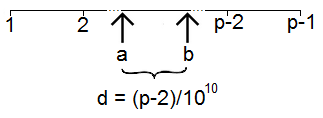
\includegraphics[width=0.5\textwidth]{logRaten.png}
    \caption{Raten des diskreten Logarithmus’}
    \label{fig:logRaten}
  \end{figure}
\end{beispiel}

\subsection{Pohlig-Hellman-Algorithmus}
\label{sub:pohlig_hellman_algorithmus}

Wenn die Ordnung von $\Z_p^*$ in viele kleine Primfaktoren zerfällt, dann kann
man diesen Umstand zur Berechnung des diskreten Logarithmus nutzen und diese
beschleunigen.

Sei $p-1 = \prod\limits_q q^k$ die Primfaktorzerlegung der Gruppenordnung von
$\Z_p^*$. Zunächst berechnen wir die $q$-ten Einheitswurzeln vom erzeugenden
Element $g$:
\begin{align*}
  r_{q, j} &
    \equiv g^{\frac{j(p-1)}{q}} \Mod{p} &
    \text{ für alle } j = 0, 1, \ldots, q-1
\end{align*}

Wir müssen nun das $x \in \Z_p^*$ finden, für das $g^x \equiv y \Mod{p}$ gilt.
Mit der Primfaktorzerlegung von $p-1$ brauchen wir nur $x \Mod{q^k}$ für jeden
Primfaktor $q$ von $p-1$ zu bestimmen, da sich $x$ dann aus dem Chinesischen
Restsatz ergibt. Wir fixieren jetzt einen Primfaktor $q$ von $p-1$ und zeigen,
wie sich daraus die Kongruenz $x \Mod{q^k}$ ergibt.

Angenommen
\begin{align*}
  x & \equiv x_0 + x_1 q + \cdots + x_{k-1} q^{k-1} \mod q^k
    & \text{ mit } 0 \leq x_i < q
\end{align*}
Für $x_0$ berechnen wir $y^{\frac{p-1}{q}}$. Da $y^{p-1} \equiv 1 \Mod{p}$,
erhalten wir eine $q$-te Wurzel von $1$. Aus $y = g^x$ folgt
\begin{align*}
  y^{\frac{p-1}{q}} &
    = g^{\frac{x(p-1)}{q}}
    = g^{\frac{x_0 (p-1)}{q}}
    = r_{q, x_0}
\end{align*}
Also vergleichen wir $y^{\frac{p-1}{q}}$ mit den zuvor berechneten Wurzeln
$r_{q, j}$ und setzen $x_0$ auf den Wert von $j$ für den
$y^{\frac{p-1}{q}} = r_{q, j}$ gilt.

Um danach $x_1$ zu finden, ersetzen wir $y$ durch $y_1 = \frac{y}{g^{x_0}}$,
denn $y_1$ hat dann den disk. Logarithmus
\begin{align*}
  x - x_0 \equiv x_1 q + \cdots + x_{k-1} q^{k-1} \mod q^k
\end{align*}
Da $y_1$ eine Potenz von $q$ ist, erhalten wir
$y_1^{\frac{p-1}{q}} \equiv 1 \Mod{p}$ und
\begin{align*}
  y_1^{\frac{p-1}{q^2}} &
    = g^{\frac{(x-x_0) (p-1)}{q^2}}
    = g^{\frac{(x_1 + x_2 q + \cdots) (p-1)}{q}}
    = g^{\frac{x_1 (p-1)}{q}}
    = r_{q, x_1}.
\end{align*}
Also vergleichen wir $y_1^{\frac{p-1}{q^2}}$ mit den berechneten Wurzeln
$r_{q, j}$ und setzen $x_1$ auf den Wert von $j$ für den
$y_1^{\frac{p-1}{q^2}} = r_{q, j}$ gilt.

Dieses Verfahren setzen wir induktiv fort. Für jedes $i = 1, 2, \ldots, k-1$
setzen wir
\begin{align*}
  y_i & = \frac{y}{g^{x_0 + x_1 q + \cdots x_{i-1} q^{i-1}}}.
\end{align*}
Dieses $y_i$ hat den disk. Logarithmus
$x_i q^i + \cdots + x_{k-1} q^{k-1} \Mod{q^k}$. Da $y_i$ eine Potenz von $q^i$
ist, erhalten wir $y_i^{(p-1)/q^i} \equiv 1$ und
\begin{align*}
  y_i^{\frac{p-1}{q^{i+1}}} &
    = g^{\frac{(x_i + x_{i+1} q + \cdots) (p-1)}{q}}
    = g^{\frac{x_i (p-1)}{q}}
    = r_{q, x_i}
\end{align*}
Wir setzen $x_i$ auf den Wert von $j$ für den
$y_i^{\frac{p-1}{q^{i+1}}} = r_{q, j}$ ist.

Abschließend erhalten wir die Kongruenz $x \Mod{q^k}$. Wenn wir dieses Verfahren
für jeden Primfaktor von $p-1$ durchgeführt haben, nutzen wir den Chinesischen
Restsatz um $x$ zu bestimmen. Algorithmus~\ref{alg:dlog_ph} beschreibt die
Vorgehensweise in Pseudocode.

\begin{beispiel}[Pohlig-Hellman-Algorithmus]
  Wir betrachten $\Z_p^*$ mit $p = 1801$ und dem Erzeuger $g = 13$. Gesucht ist
  jenes $x$ mit $g^x \equiv 111 \Mod{p}$. Die Primfaktorzerlegung von $p-1$ ist
  $2^3 \cdot 3^2 \cdot 5^2$.

  Wir bestimmen zunächst die Einheitswurzeln
  $r_{q, j} \equiv g^{\frac{j(p-1)}{q}} \Mod{p}$ zu jedem Primfaktor $q$:
  \begin{center}
    \begin{tabular}{rrrrrr}
      \toprule
      $j$ & $0$ & $1$ & $2$ & $3$ & $4$\\
      \midrule
      $r_{2,j}$ & $1$ & $1800$\\
      \midrule
      $r_{3,j}$ & $1$ & $1727$ & $73$\\
      \midrule
      $r_{5,j}$ & $1$ & $350$ & $32$ & $394$ & $1024$\\
      \bottomrule
    \end{tabular}
  \end{center}
  Wir beginnen mit dem Primfaktor $q = 2$ und müssen $x \Mod{2^3}$ finden. Wir
  schreiben dieses $x$ als $x_0 + 2 x_1 + 4 x_2$. Für $x_0$ berechnen wir
  $111^{1800/2} \equiv 1 \Mod{1801}$. In der zuvor berechneten Tabelle der
  Einheitswurzeln schauen wir nach, für welches $j$ der Wert von $r_{2, j} = 1$
  ist. Dies ist für $j=0$ der Fall, also ist $x_0 = 0$. Danach berechnen wir
  $111^{1800/4} \equiv 1 \Mod{1801}$, also ist auch $x_1 = 0$. Zuletzt
  berechnen wir $111^{1800/8} \equiv 1 \Mod{1801}$, woraus $x_2 = 0$ folgt.
  Damit erhalten wir unsere erste Kongruenz:
  \begin{align*}
    x \equiv 0 + 2 \cdot 0 + 4 \cdot 0 \equiv 0 \mod 8
  \end{align*}
  Wir fahren fort mit $q = 3$. Das gesuchte $x$ wird dabei als $x_0 + 3 x_1$
  geschrieben. Für $x_0$ berechnen wir $111^{1800/3} \equiv 1727 \Mod{1801}$,
  sodass $x_0 = 1$ ist. Da jetzt ein Koeffizient $\neq 0$ aufgetreten ist,
  müssen wir $111$ durch $g^{x_0}$ teilen. Dazu bestimmen wir das multiplikative
  Inverse von $g = 13$ modulo $p = 1801$ mit dem erweiterten Euklidischen
  Algorithmus: $g^{-1} = 1524$. Für $x_1$ rechnen wir
  ${(111 \cdot 1524)}^{1800/9} \equiv 1727 \Mod{1801}$, sodass auch $x_1 = 1$
  ist. Dies ergibt die Kongruenz:
  \begin{align*}
    x \equiv 1 + 3 \cdot 1 \equiv 4 \mod 9
  \end{align*}
  Für die letzte Kongruenz schließen wir ab mit $q = 5$. Wir beginnen mit $x_0$
  und berechnen $111^{1800/5} \equiv 394 \Mod{1800}$, woraus $x_0 = 3$ folgt.
  Für $x_1$ berechnen wir
  ${\left(111 \cdot 1524^3\right)}^{1800/25} \equiv 394 \Mod{1801}$
  und erhalten $x_1 = 3$, sodass unsere letzte Kongruenz
  \begin{align*}
    x \equiv 3 + 5 \cdot 3 \equiv 18 \mod 25
  \end{align*}
  lautet. Diese Kongruenzen lassen sich mit dem Chinesischen Restsatz lösen und
  wir erhalten
  \begin{align*}
    x \equiv 1768 \mod 1801
  \end{align*}
  als Lösung. Die Probe $13^{1768} \equiv 111 \mod 1801$ bestätigt dies.
\end{beispiel}

\listoffigures

\begin{thebibliography}{9}
  \bibitem{koblitz94}
    Neal Koblitz,
    \textit{A course in number theory and cryptography},
    Springer,
    2. Auflage,
    1994.

  \bibitem{forster2015}
    Otto Forster,
    \textit{Algorithmische Zahlentheorie},
    Springer Spektrum,
    2. Auflage,
    2015

  \bibitem{HAC97}
    Menezes, Alfred,
    Oorschot, Paul C.,
    Vanstone, Scott A.,
    \textit{Handbook of applied cryptography},
    CRC Press,
    1 edition,
    1996
\end{thebibliography}

\end{document}
